\begin{figure}[H]
	\centering
	\begin{subfigure}{0.5\columnwidth}
		\centering
		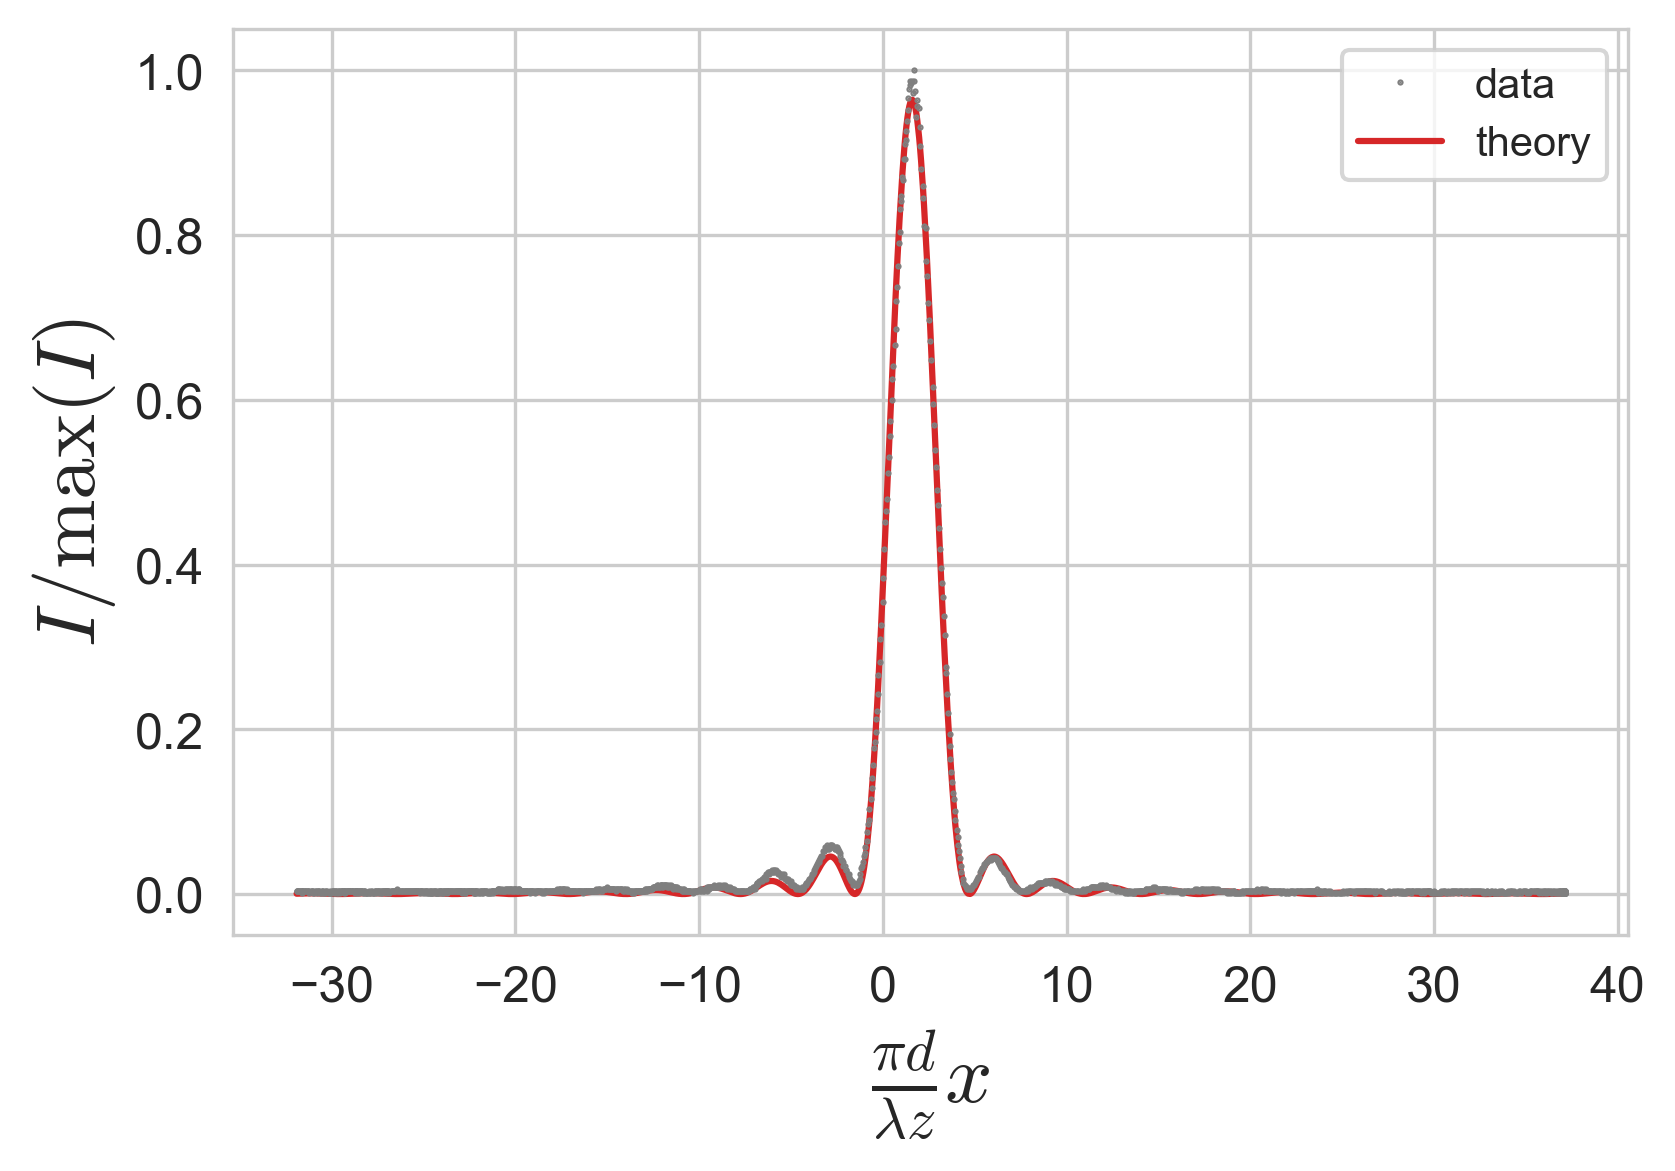
\includegraphics[width=\columnwidth]{figures/single slit interference 0.08mm.png} % first figure itself
		\caption{}
        \label{fig:single slit interference 0.08mm}
	\end{subfigure}\hfill
    \begin{subfigure}{0.5\columnwidth}
        \centering
        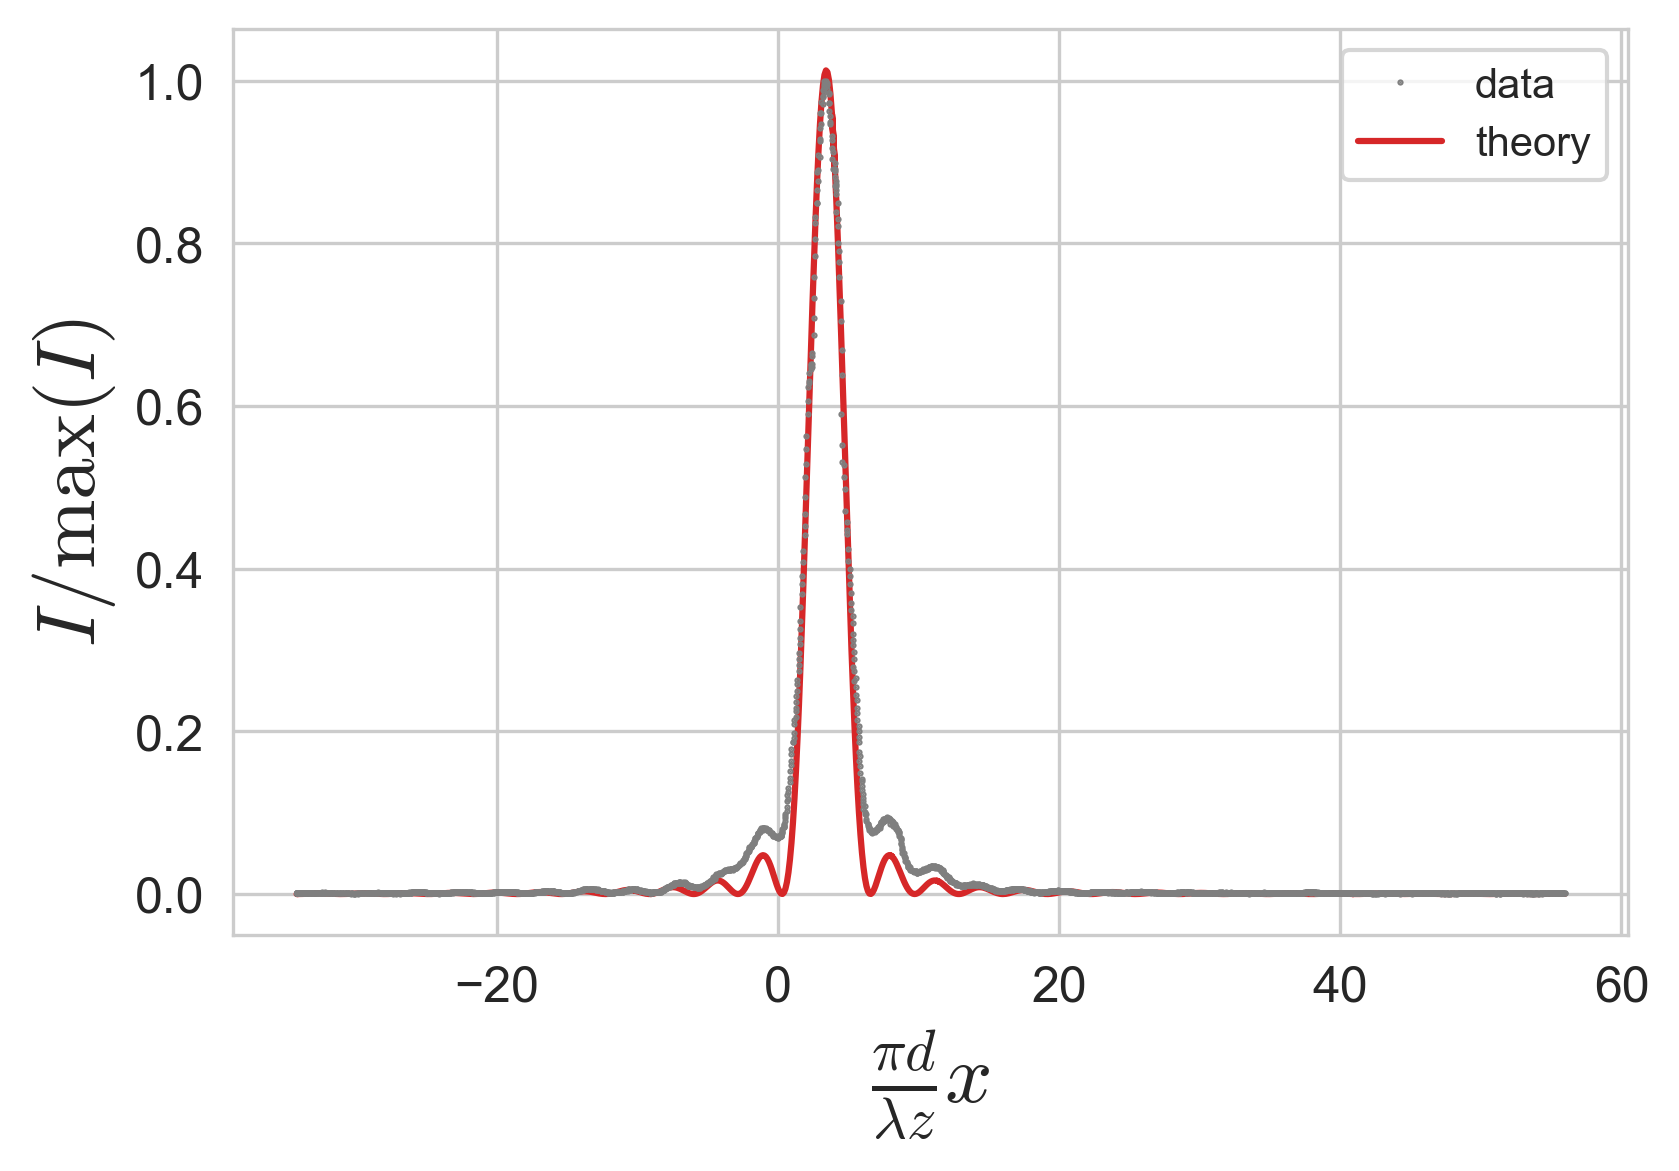
\includegraphics[width=\columnwidth]{figures/single slit interference 0.16mm.png} % second figure itself
        \caption{}
        \label{fig:single slit interference 0.16mm}
    \end{subfigure}
    \begin{subfigure}{0.5\columnwidth}
        \centering
        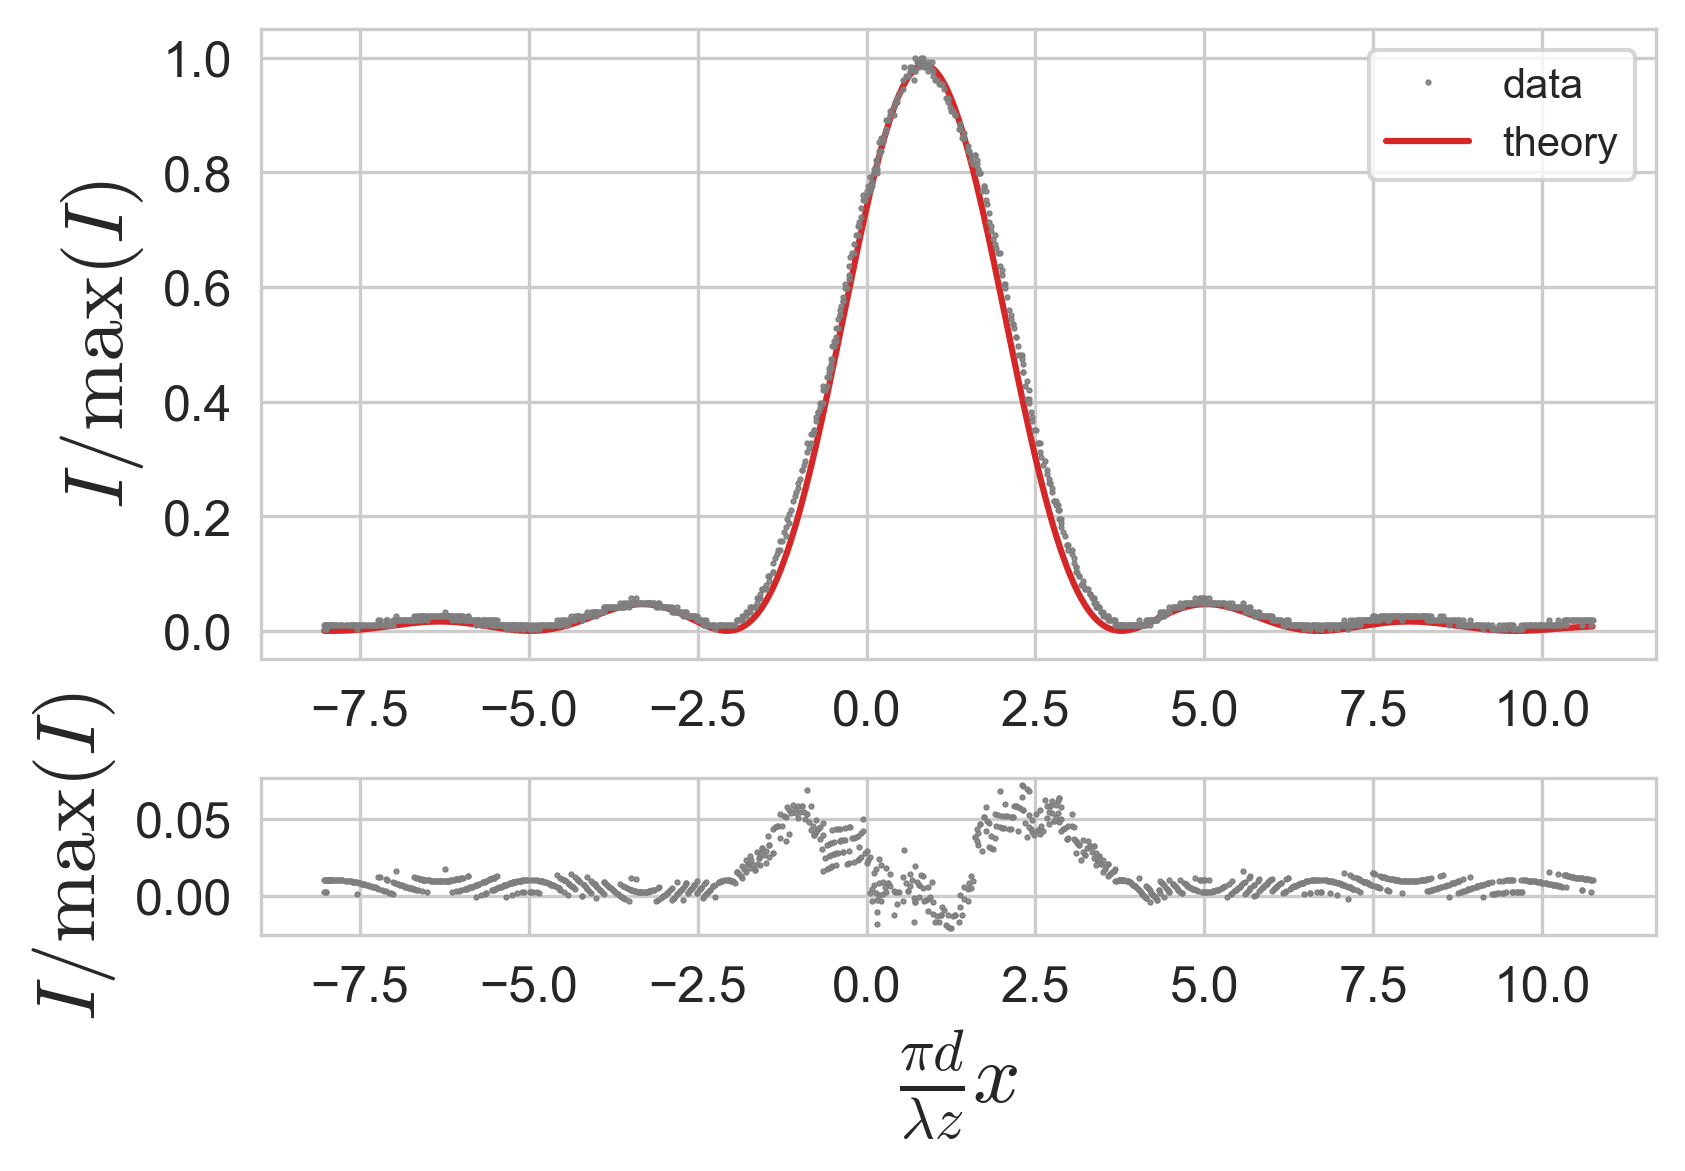
\includegraphics[width=\columnwidth]{figures/single slit interference with 0.04mm not best fit but better tails.png}
        \caption{this figure is used to show with greater clarity the secondary effects in the tails of the interference pattern residuals graph}
        \label{fig:single slit interference with 0.04mm not best fit but better tails}
    \end{subfigure}
    \label{fig:single slit examples}
\end{figure}
